% !TEX root = ../main.tex

\chapter{Phase 1 - Data Collection}

\section{Objectives}

The objective of the first phase is to establish a reliable and reproducible dataset that serves as the empirical foundation for the subsequent
stages of the project. Since the validity of any data-driven analysis depends fundamentally on the quality and consistency of the underlying data,
this phase focuses on collecting, organising and preparing relevant information from the selected Upwork marketplace categories.

The outcome of this phase is a structured dataset containing publicly available job information related to selected
Python-related data freelance categories, including data analysis, data engineering, Python automation and machine learning.
The resulting dataset is prepared for exploratory data analysis and provides the basis for answering the research questions
introduced in Chapter~1.

\section{Scope of the Dataset}

The scope of the dataset was deliberately limited to a selected segment of the Upwork marketplace consisting of Python-related data freelance
jobs. Rather than analysing the entire marketplace, the study focuses on categories including data analysis, data engineering,
Python automation and machine learning. This targeted scope allows the analysis to concentrate on a coherent group of closely related professional
domains while remaining directly relevant to the objectives of the project.

The final dataset contains 44 manually collected Upwork job postings gathered during July 2026. Each job was stored as an individual
text file containing the complete textual content of the corresponding job posting together with additional metadata, including the original job URL,
the selected search category and the search keyword used during data collection. Preserving the complete job descriptions ensured that
all potentially relevant information remained available throughout the subsequent stages of preprocessing and analysis.

The relatively small size of the dataset reflects the current limitations of publicly accessible Upwork data rather than a limitation of
the developed data collection workflow. Since direct programmatic access to the Upwork platform was not available, each job posting had to be collected manually.
Nevertheless, the developed data collection pipeline was intentionally designed in a modular manner. With only minor modifications to
its initial acquisition stage, the same workflow could be applied to substantially larger datasets if direct access to the Upwork API or
another automated data source became available in the future.

\section{Data Collection Procedure}

The data collection process began by identifying relevant job postings within the selected Upwork categories. Jobs related to data analysis,
data engineering, Python automation and machine learning were located using the Upwork search interface and predefined search terms corresponding to
the scope of the study. Each selected job was then individually reviewed to determine whether it matched the objectives of the dataset.

Since direct programmatic access to the Upwork platform was not available, each job was collected manually. The complete textual content of
every selected job posting was copied into an individual plain text file, preserving the original structure of the advertisement.
In addition to the job description, each file contained supplementary metadata such as the original job URL, the selected marketplace category
and the search keyword used during data collection.

Rather than extracting only predefined variables during data collection, the complete job descriptions were preserved.
This approach ensured that no potentially relevant information was discarded at an early stage and allowed the preprocessing pipeline to
identify additional technologies, software tools, programming libraries and technical skills directly from the original job descriptions.

The adopted collection procedure separates raw data acquisition from subsequent preprocessing and analysis. As a result, the original job postings
remain permanently available for verification, while improvements to the preprocessing pipeline can be applied repeatedly without
requiring the data collection process to be repeated. This modular workflow improves the reproducibility and maintainability of the entire project.

\begin{figure}[H]
    \centering
    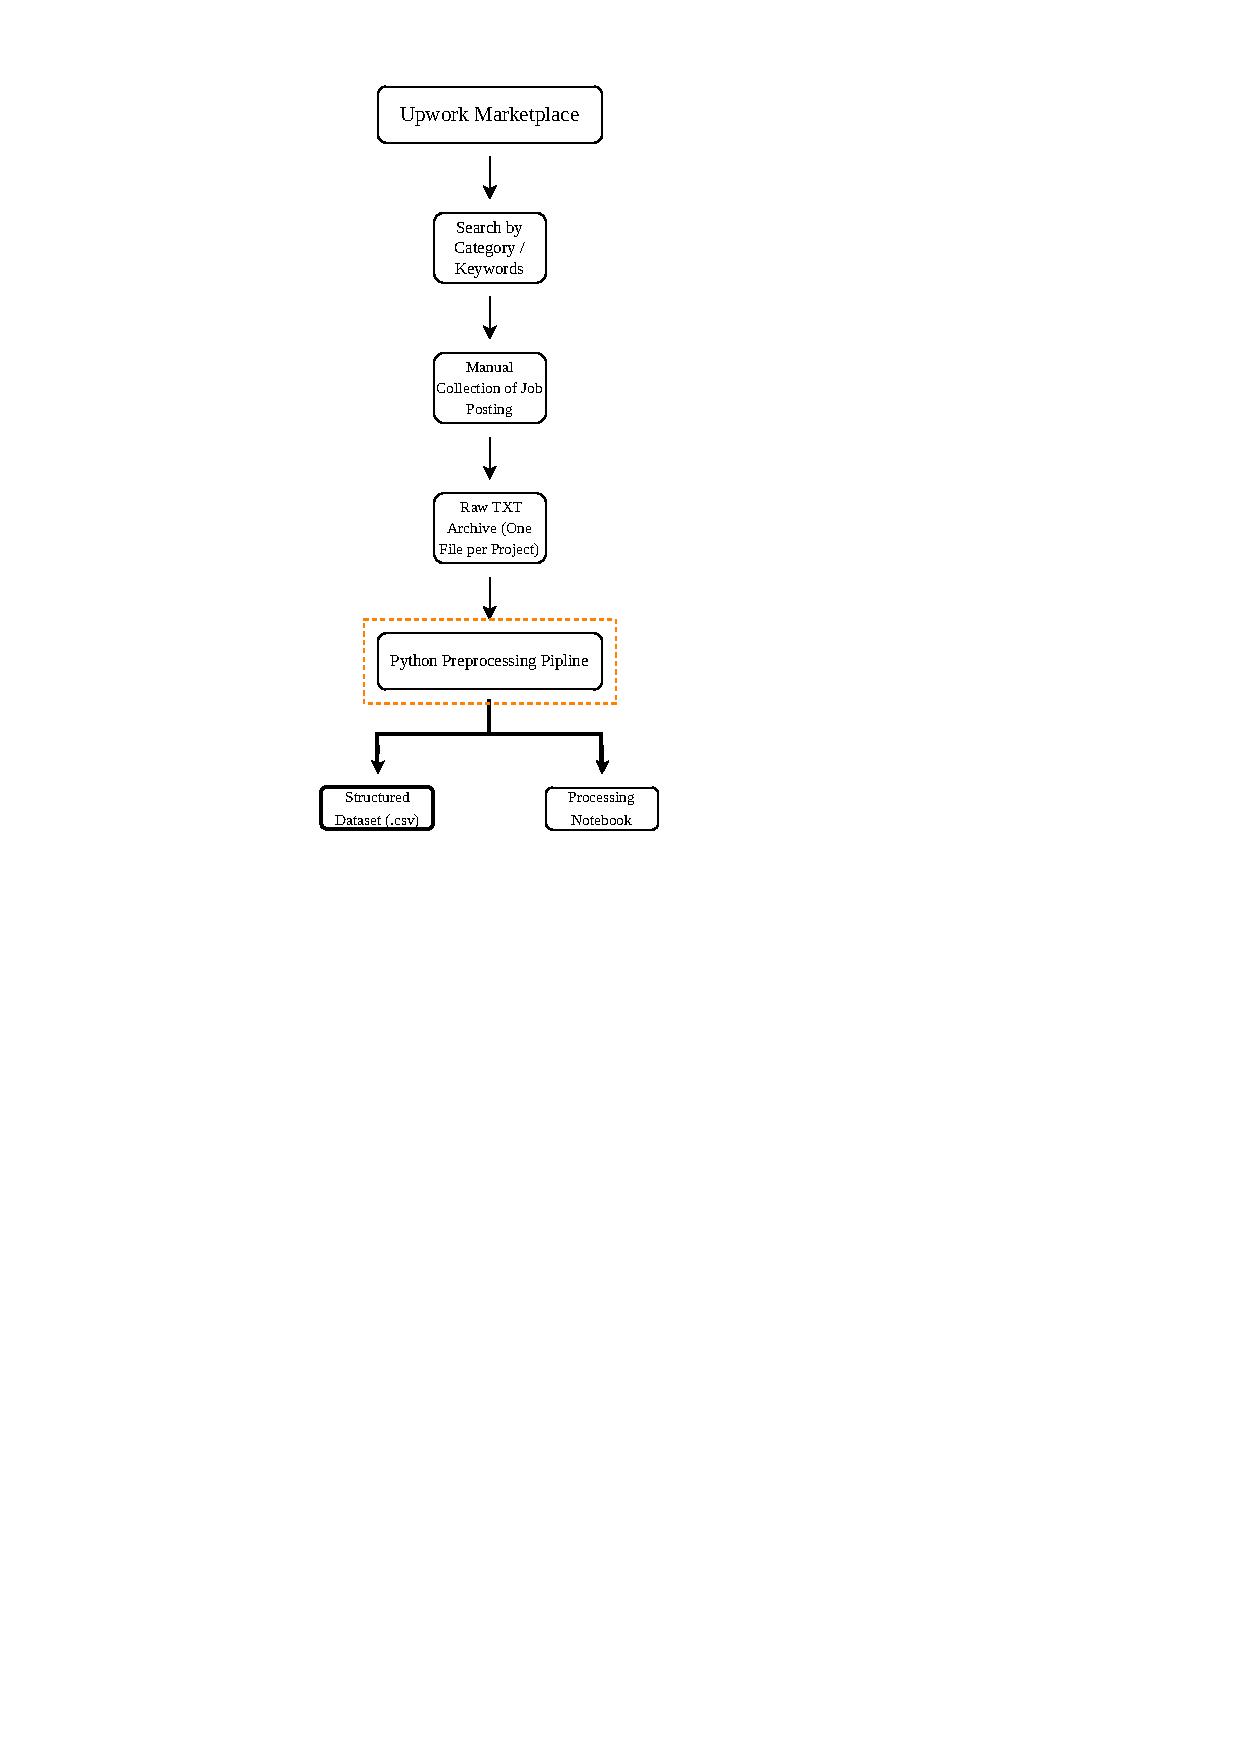
\includegraphics[
    width=0.8\textwidth,
    trim=4cm 14cm 8cm 0cm, %left, bottom, right, top
    clip
    ]{figures/workflow/phase1_pipeline.pdf}
    \caption{Overview of the data collection workflow.}
    \label{fig:phase1_pipeline}
\end{figure}

\section{Dataset Structure}

Following the data collection procedure, the raw text archive was transformed into a structured dataset suitable for automated analysis.
During this process, relevant information was extracted from each job posting and organised into a tabular format, where each row represents a
single Upwork job and each column corresponds to a specific job attribute. The resulting structure enables efficient filtering,
statistical analysis and visualisation while preserving the information required to answer the research questions introduced in Chapter~1.

\begin{table}[H]
\centering
\caption{Structure of the final dataset.}
\label{tab:dataset_structure}

\begin{tabularx}{\textwidth}{l l X}
\toprule
\textbf{Variable} & \textbf{Type} & \textbf{Description} \\
\midrule
job\_id & Integer & Unique identifier assigned to each collected job. \\

category & Categorical & Upwork marketplace category from which the job was collected. \\

search\_keyword & String & Search keyword used during data collection, if applicable. \\

title & String & Title of the job posting. \\

description & Text & Complete textual description of the project. \\

mandatory\_skills & Text & Technical skills explicitly required by the client. \\

preferred\_qualifications & Text & Skills or qualifications listed as desirable but not mandatory. \\

experience\_level & Categorical & Client's requested experience level. \\

job\_type & Categorical & Hourly or fixed-price job. \\

project\_type & Categorical & Type of project (e.g. ongoing project). \\

duration & String & Expected project duration. \\

workload & String & Expected weekly workload. \\

budget\_type & Categorical & Representation of the available budget information. \\

budget\_min & Numeric & Lower budget bound or hourly rate. \\

budget\_max & Numeric & Upper budget bound or hourly rate. \\

posted\_date & String & Relative publication date shown on Upwork. \\

proposals & String & Number of submitted proposals. \\

job\_url & String & Original URL of the Upwork job posting. \\

collected\_at & DateTime & Timestamp indicating when the job was collected. \\
\bottomrule
\end{tabularx}
\end{table}

The dataset combines unstructured textual information with structured metadata extracted from each job posting. While the textual fields
preserve the original content required for keyword extraction and qualitative analysis, the structured variables provide the basis for
statistical analyses, filtering and visualisation throughout the subsequent stages of the project.

\section{Data Cleaning and Preprocessing}

Although the manually collected text files contained all information required for the subsequent analysis, the data were stored as unstructured
text and therefore required preprocessing before quantitative analysis could be performed. The primary objective of this stage was to transform
the raw text archive into a consistent, structured dataset while preserving the original job information.

A Python-based preprocessing pipeline was developed to automate the extraction of relevant job attributes from each text file.
Individual extraction functions were implemented for all major project characteristics, including the job title, category, job description,
required skills, experience level, project type, budget information, workload, duration, proposal statistics and the original job URL.
This modular design improves the maintainability of the preprocessing pipeline while also allowing it to be extended or adapted to future changes in
the structure of Upwork job postings. The extracted values were subsequently organised into a unified tabular structure matching the predefined
dataset schema.


Several preprocessing steps were incorporated to improve the consistency of the resulting dataset. Budget values were converted into a unified
numerical representation, categorical variables were standardised, missing values were handled explicitly where applicable, and the collected
information was validated before being exported to the final CSV dataset. Automating these operations ensured that identical processing rules
were applied to every collected job, thereby improving the reproducibility, consistency and maintainability of the entire
preprocessing workflow.

\begin{figure}[H]
    \centering
    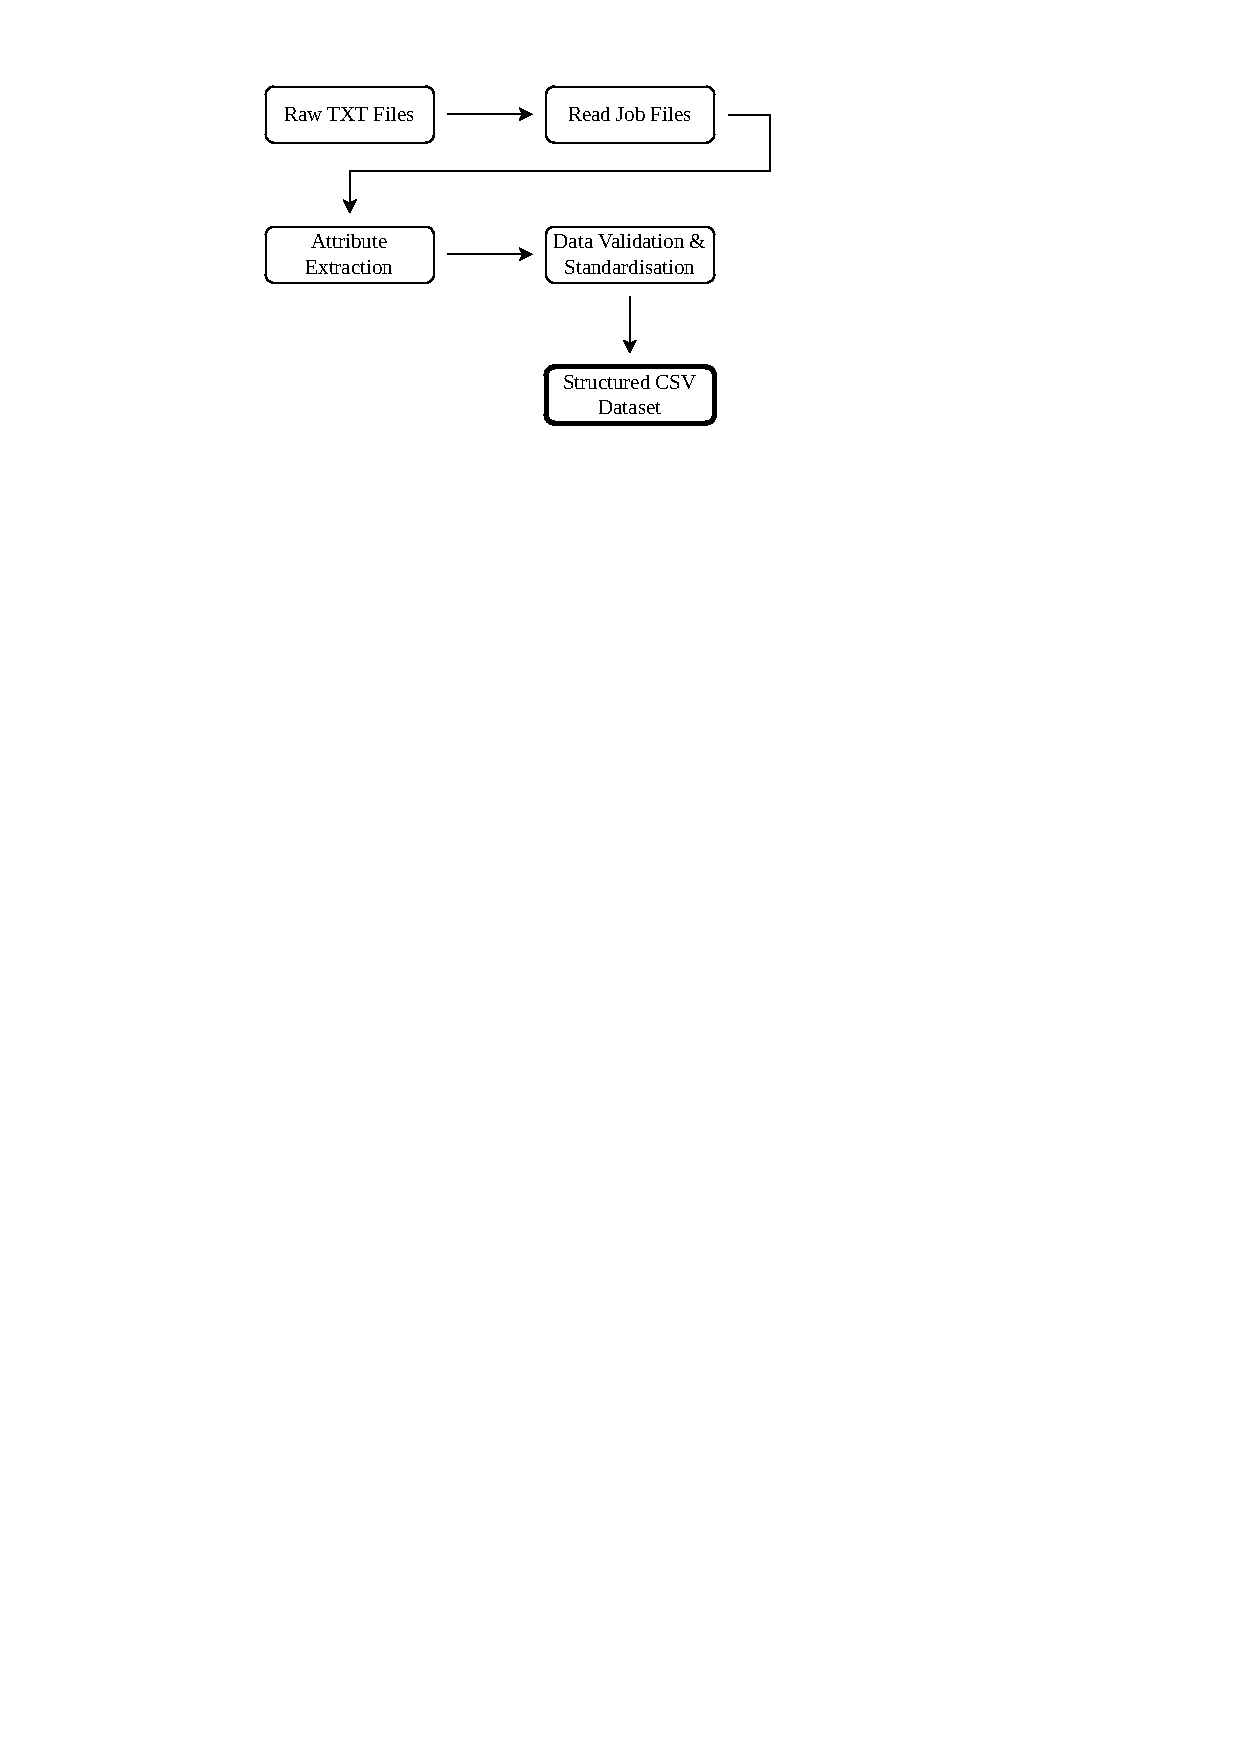
\includegraphics[
    width=1\textwidth,
    trim=0cm 22cm 4cm 0cm, %left, bottom, right, top
    clip
    ]{figures/workflow/phase1_preprocessing_pipeline.pdf}
    \caption{Overview of the preprocessing pipeline used to transform raw Upwork job postings into a structured dataset.}
    \label{fig:phase1_preprocessing_pipeline}
\end{figure}

\section[Phase 1 Summary]{Phase Summary}

The first phase of the project established a complete and reproducible workflow for collecting and preparing Upwork job postings for
quantitative analysis. Starting from manually collected raw text files, the developed preprocessing pipeline transformed unstructured
job descriptions into a structured dataset containing both textual information and standardised job attributes.
Throughout this phase, particular emphasis was placed on data consistency, modularity and reproducibility, ensuring that
the resulting dataset provides a reliable foundation for subsequent analysis.

With the data collection and preprocessing stages completed, the project proceeds to exploratory data analysis.
The following chapter addresses each of the research questions introduced in Chapter~1 through descriptive statistical analyses of
the structured dataset, providing the empirical basis for the market insights and portfolio recommendations presented in the subsequent phases.